%DO NOT MESS AROUND WITH THE CODE ON THIS PAGE UNLESS YOU %REALLY KNOW WHAT YOU ARE DOING
\chapter{Design} \label{Design}
\section{Equipment \& Software used}
\subsection{Software}
\begin{enumerate}
\item \underline{Oracle  Virtualbox}

  Oracle Virtualbox is a cross platform type 2 hypervisor. It runs across windows, mac and linux and allows us to install and use guest operating systems inside virtual machines. Using a virtual machine helps in management of dependencies and creates reproducible environments which can help while prototyping. We used Virtualbox for setting up dependencies and capturing data with the help of PlutoSDR.
\newpage

\item \underline{Python}

  Python is a programming language with very powerful and easy to use libraries. It has a large set of libraries for machine learning, signal processing, among others. Since it is popular with academic and student communities, it has a large set of APIs for interfacing with various SDR.

\item \underline{Conda}

  Conda is a open source package and environments management system for Python. It maintains it's own set of libraries and has preconfigured environments for machine learning libraries such as TensorFlow. It also makes it easy to create virtual environments and use multiple versions of Python without dependency issues. We used a minimal version of conda called miniconda to install Python 3.9 and manage dependencies for PlutoSDR and TensorFlow.

\item \underline{TensorFlow}

  TensorFlow is a open source platform for machine learning. It has a large support for creating and deploying various types of neural networks along with easy to use interface though Keras. We used it for training our neural networks to distinguish between drone and non-drone signal.
\item \underline{NumPy}

  NumPy is the standard library for array related computation for Python. NumPy makes it easy to handle arrays in Python through it's vast list of modules and functions. It is relatively fast as it relies on C/C++ under the hood for the computation. It also has some handy functions for Fourier Transforms inside the fft module. 

\item \underline{Matplotlib}

  Matplotlib is the standard library for plotting and visualization of data in Python. It makes it easy to plot, add legend and annotations and export plots for various purposes. We used it primarily to plot the sampled data and PSD for the same. We also used it to visualize and interpret many of the results.
\end{enumerate}

\subsection{Hardware}
\begin{enumerate}
\item \underline{PlutoSDR}

ADALM-PLUTO is a Software Defined Radio learning module developed by Analog Devices. It is based on Analog Devices AD9363 and Xilinx\textsuperscript{\textregistered} Zynq Z-7010 FPGA. It  can scan from 325 MHz to 3.8 GHz which makes it suitable for scanning the ISM band at 2.4 GHz. It can also transmit at the same frequencies with a maximum bandwidth of 20 MHz. It connects over a standard USB3 connection as a USB ethernet controller which makes it easy to pass through to virtual machines. It also has a well documented Python library which makes it easier to use it in projects. 

\item \underline{RTLSDR}

RTLSDR is another software  Defined Radio based off of DVB-T TV tuner dongles based on the RTL2832U chipset. It is a very cheap SDR which can be used to scan RF spectrum. It's is capable of only receiving signals and not transmitting them. It can usually scan between 50 MHz to 1000 MHz with some models even able to scan till 2200 MHz. It can also use a upconverter for scanning higher bands. We primarily used it for experimenting with spectrum scanning and plotting.

\end{enumerate}
\section{Design} \label{Design}

\subsection{Creation of the Dataset}
\subsubsection*{ Data Capture}

\noindent During this stage, we undergo the process of capturing the RF energy signatures of drones or any other RF devices in the vicinity using a RF receiver.

\noindent This stage can be divided into three sections:
\begin{enumerate}
  \item Set up
  \item Receiver Calibration
  \item Signal Detection
\end{enumerate}
%change set up to setup
\begin{figure}[H]
  \centering
  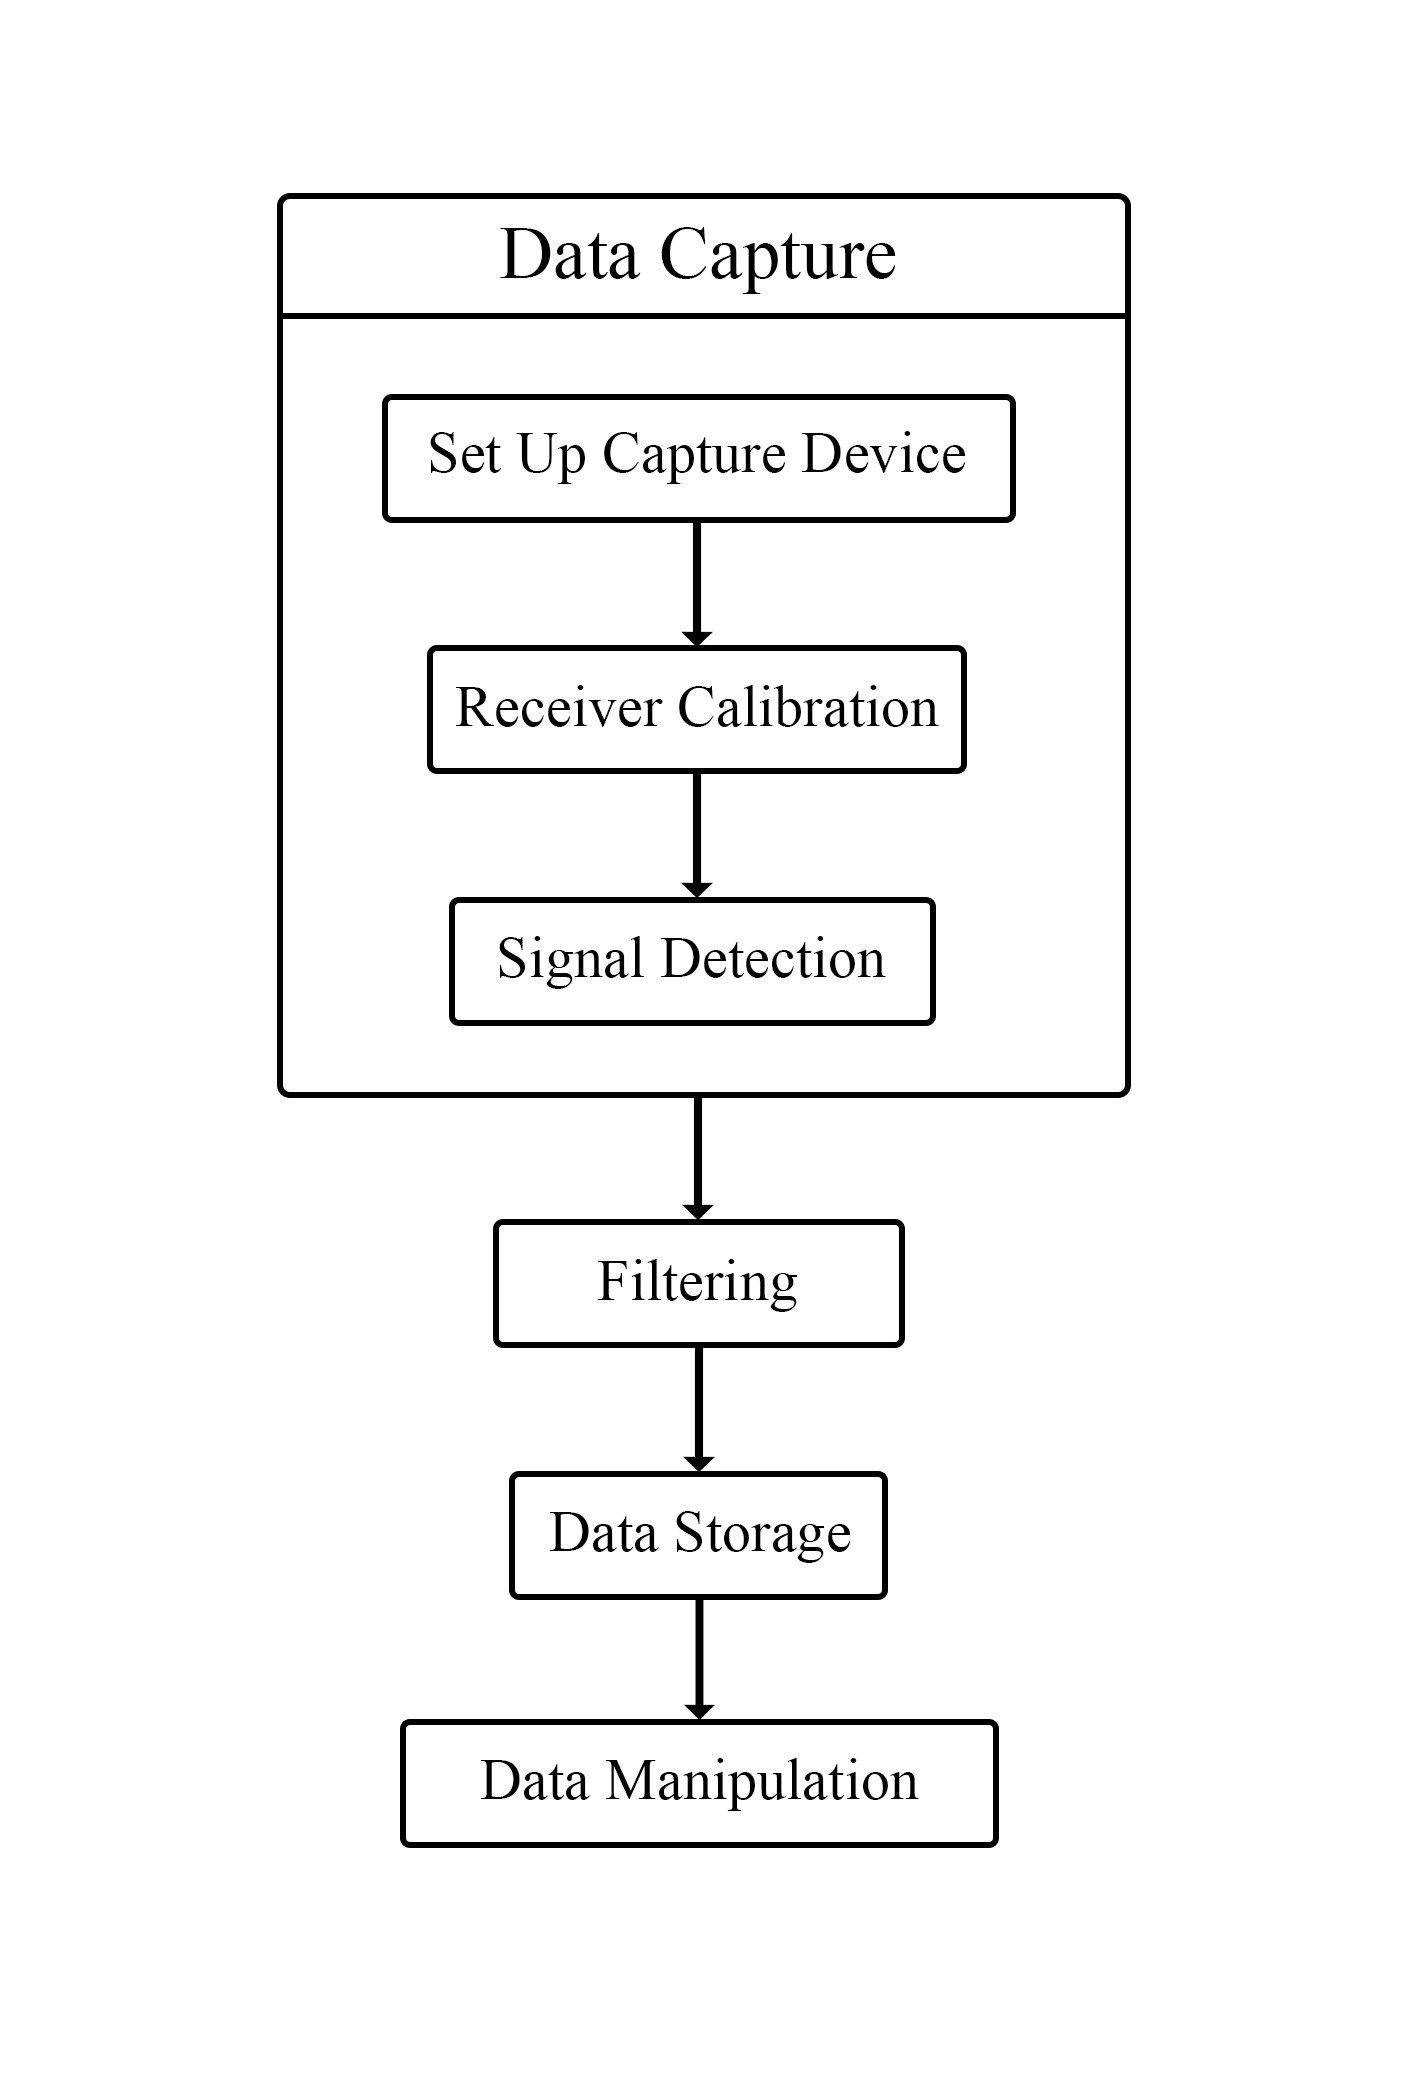
\includegraphics[width=0.5\textwidth]{Data creation.png }
  \caption{Data creation pipeline}
\end{figure}

%set up
\begin{enumerate}
  \item \underline{Set up}
    \begin{itemize}
      \item To begin with the data capture process, we require to install Python 3.9 as given in Appendix-0.1. Then import the appropriate libraries and APIs for PlutoSDR, Matplotlib libraries, and NumPy libraries in Python after following appropriate steps to install TensorFlow via Conda as shown in Appendix-0.1.
    \end{itemize}

    % rx calibration
  \item \underline{ Receiver calibration}
    \begin{itemize}
      \item We require to import the appropriate Python libraries and APIs for PlutoSDR to initialize its functional parameters such as scan bandwidth, sampling rate, RF bandwidth, and sample capturing functionalities.
      \item During this Stage, we ensure to calibrate the Receiver parameters properly to produce the required signal outputs for the training and evaluation stages.
    \end{itemize}


  \item \underline{ Signal Detection}
    \begin{itemize}
      \item Using PlutoSDR as a receiver, a time frame of 5 sec is taken for a  scan range of 2.405-2.715 GHz with a scan bandwidth of 2.5MHz. The recorded points are the FFT energy readings for corresponding frequency components in the time frame of 5 seconds and are stored in tuple data type. This is achieved using the Python libraries of PlutoSDR, math(filter design).
      \item To facilitate filtering action ahead, these tuples are then converted to NumPy array to allow data manipulation.
    \end{itemize}
\end{enumerate}


\subsubsection*{Filtering}
\begin{itemize}
  \item During dataset creation to remove noise and unwanted signals due to various natural reasons (ambient noise \& natural resonance of SDR etc), a threshold of 15,000 in energy level is set. This helps in lowering dataset size by removing noise signals and replacing them with 0. ie. any signal greater than 15,000 in energy level are recorded as they are, while others are substituted with '0' in the training dataset while storing them.

  \item This concept is further utilized to ensure that valid scan time signals are recorded and ideal no-signal scanning values are discarded to ensure proper dataset creation.

  \item Following this, the recorded signals are manipulated appropriately and passed to the next process block.
\end{itemize}

\subsubsection*{Data Storage}
\begin{itemize}
  \item During dataset storage, the recorded signals present in the NumPy array are converted into a Pandas DataFrame using the Pandas library in Python for easy access and storage.
  \item During the storage process, we have to ensure to include the parameter 'index=False' in the 'store.to\_csv' command to remove the storage of the array indices in the resultant CSV files.
  \item These files are further utilized either for training or evaluation, depending on the process cycle of the project.
\end{itemize}


\subsubsection*{Data Manipulation}
\begin{itemize}
  \item This stage is only applicable in the training dataset preparation process to create a training dataset. We have recorded multiple signals and stored them independently resulting in a large set of CSV files. Multiple CSV files are generated by multiple capture runs and fragmentation of the frequency spectrum due to limited capture range while capturing a wide bandwidth.
  \item In this stage, multiple CSV files are combined to form a larger file with an additional data row which provides training labels that are utilized in the machine learning training process. In this case, training label ‘0’ is for the non-drone signals while ‘1’ is for the drone signals.
  \item A singular dataset file is generated containing different ratios of drone and non-drone signals. This is done by appending multiple random drone and non-drone signals with their training labels and shuffling them by using numpy.random.shuffle function.


\end{itemize}

\subsection{Training the model}
\begin{figure}[H]
  \centering
  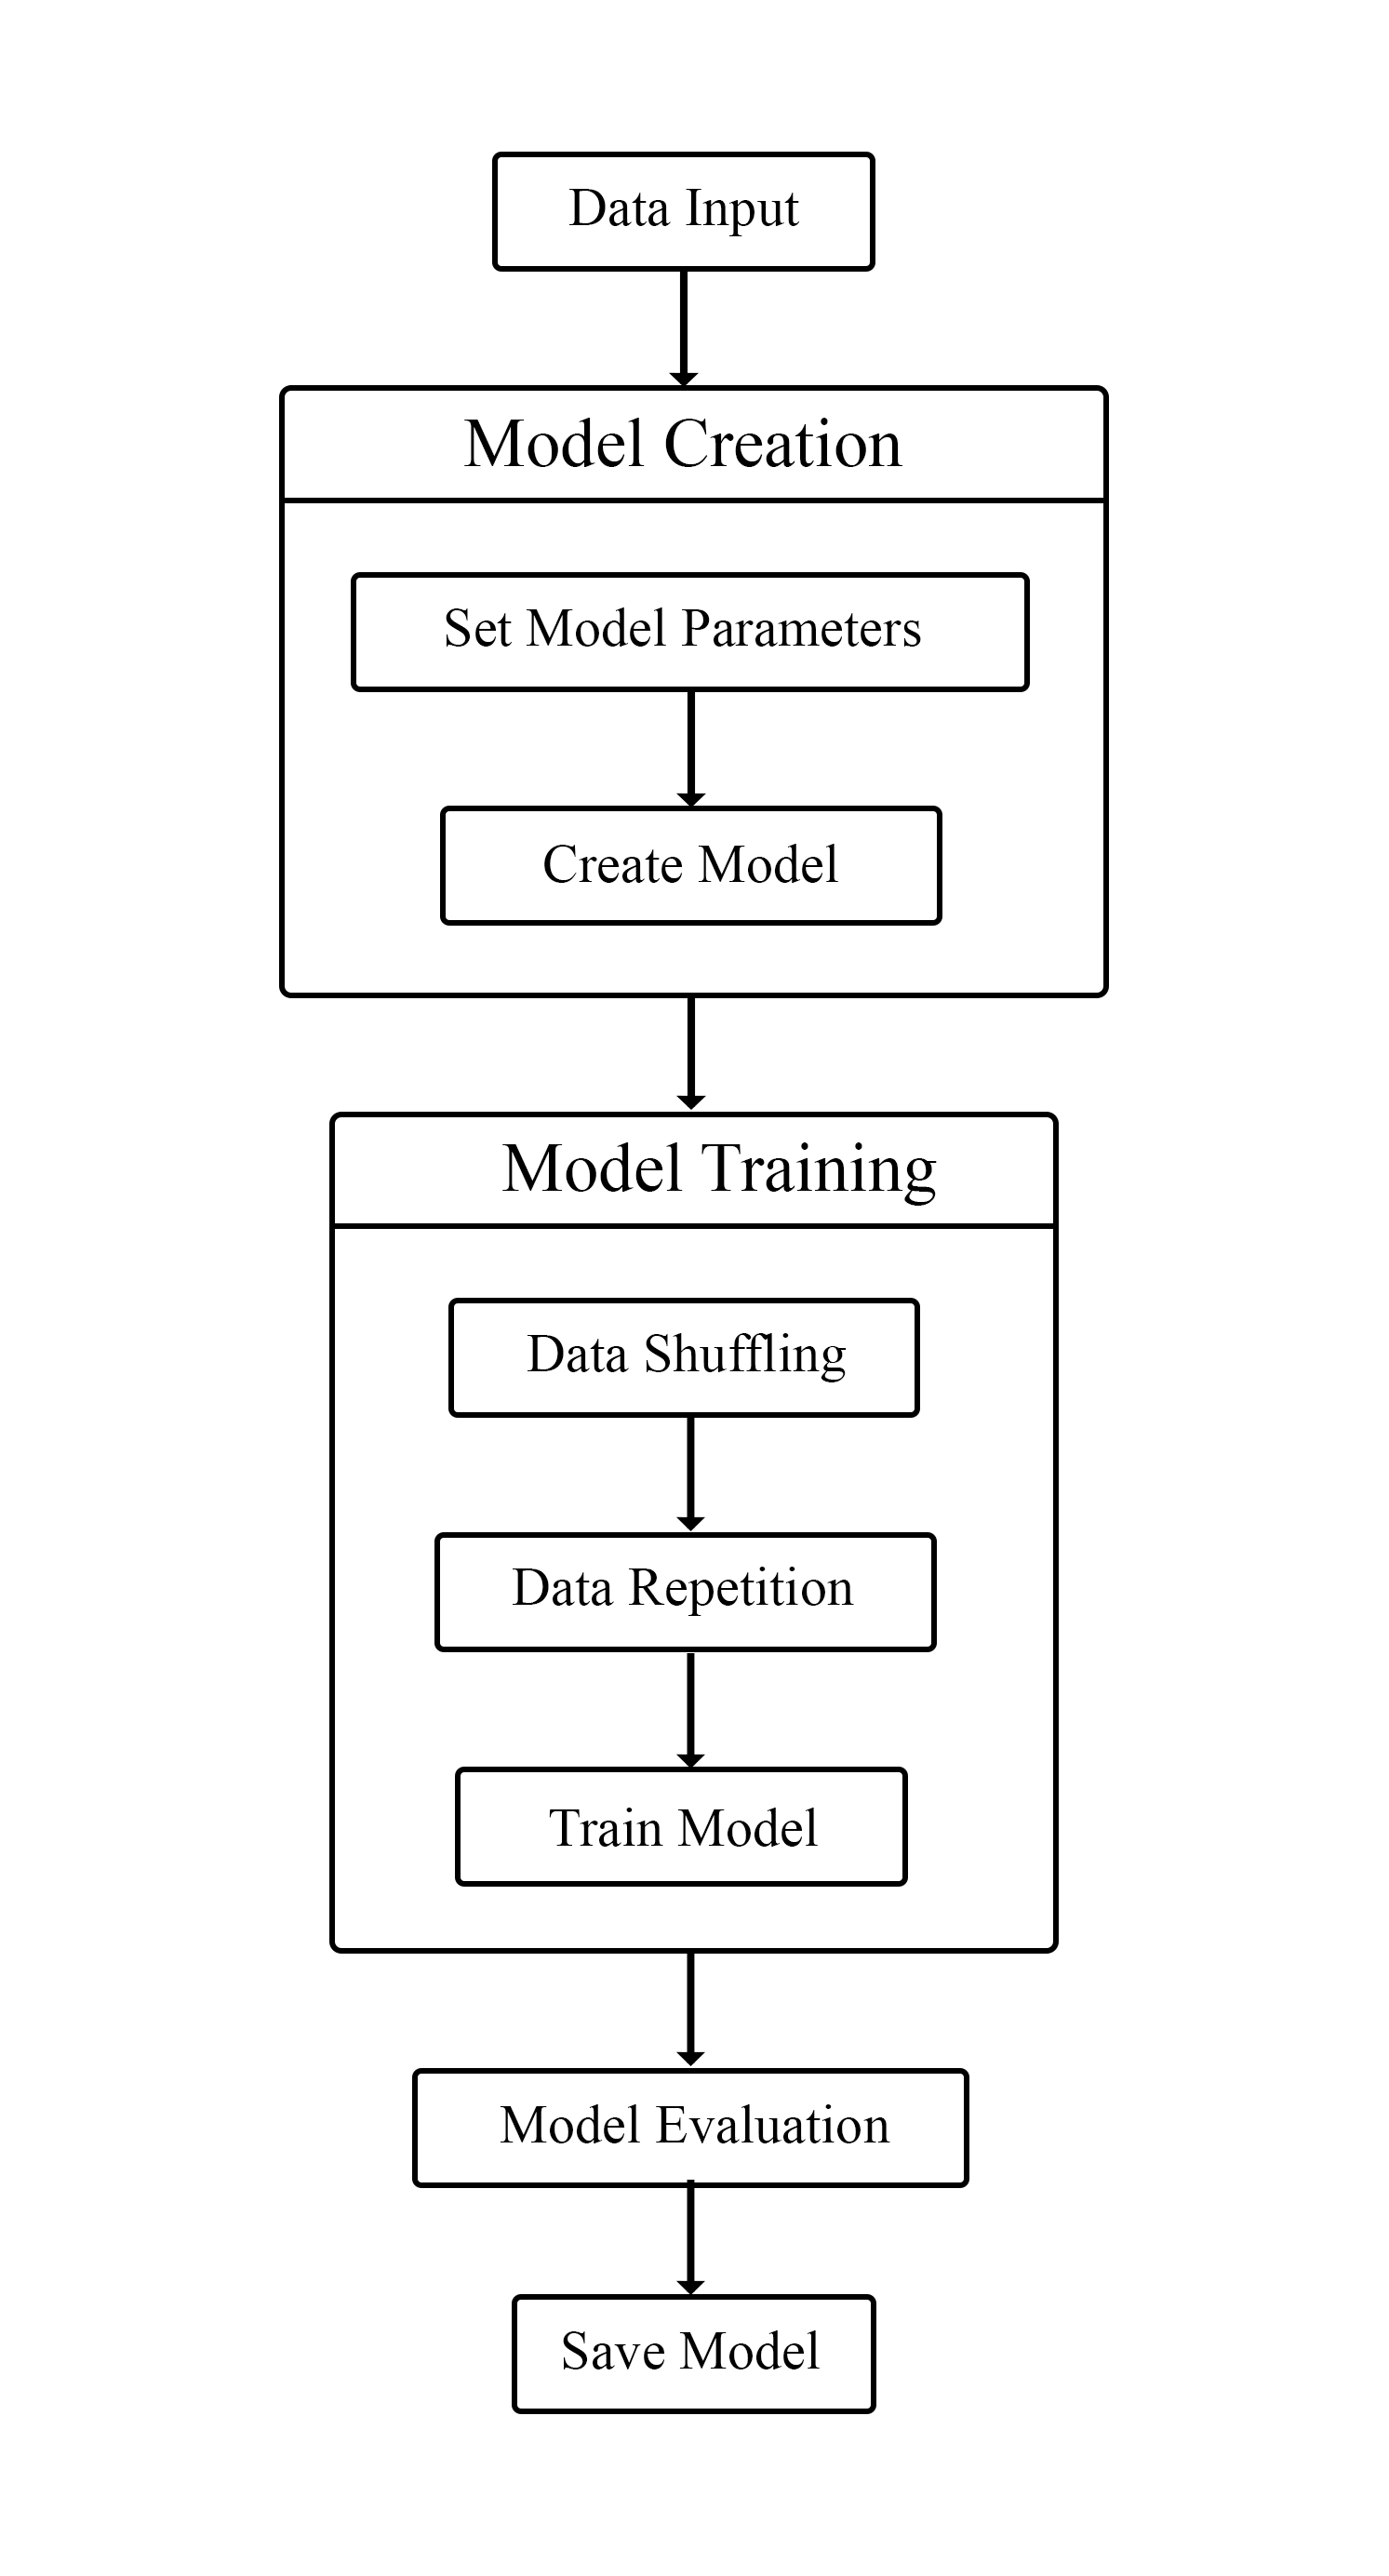
\includegraphics[width=0.5\textwidth]{ML training.png}
  \caption{Model Creation Pipeline}
\end{figure}

\subsubsection*{1.Data Input}
\begin{itemize}
  \item   To begin with the training process, we load the stored training dataset stored in .csv format into the system memory in the form of a Pandas DataFrame.
  \item For training, the DataFrame is divided into two parts namely 'train\_labels' and 'train\_features'. Where the test\_labels are used for training validation and test\_features refer to the input data on which the model is to be trained on.
  \item train\_features undergo a normalization process to ensure proper learning parameters are extracted from the input data.
  \item Further, these two parts are then joined appropriately forming a tensor dataset named 'train\_dataset' which is later given to the training model.
\end{itemize}

\subsubsection*{2.Model creation}
During this stage, we undergo the processes involved in the creation of a model which is to be trained later on.

\noindent This stage can be divided into two sections:
\begin{enumerate}
  \item Model Parameters
  \item Creating the model
\end{enumerate}

\begin{itemize}
  \item \underline{Model Parameters}
    \begin{itemize}
      \item During this stage, the model parameters such as the number of layers, types of layers used, type of activation functions associated with the model layers are declared and initialized.
      \item In our application, we have made use of sequential model available under keras.
    \end{itemize}
  \item \underline{Model Creation}
    \begin{itemize}
      \item In model creation, it includes declaration and initialization of the model parameters shown in the prior sections and it also involves the definition and declaration of other model parameters such as its loss function, metrics, and optimizer function
      \item The later stated parameters are used during the training process to change the layer weights and strengths associated with hidden layer nodes of the model as and when required for proper training and learning gradient calculation, while metrics are provided for analysis of the model by the user.
    \end{itemize}
\end{itemize}
\begin{figure}[H]
  \centering
  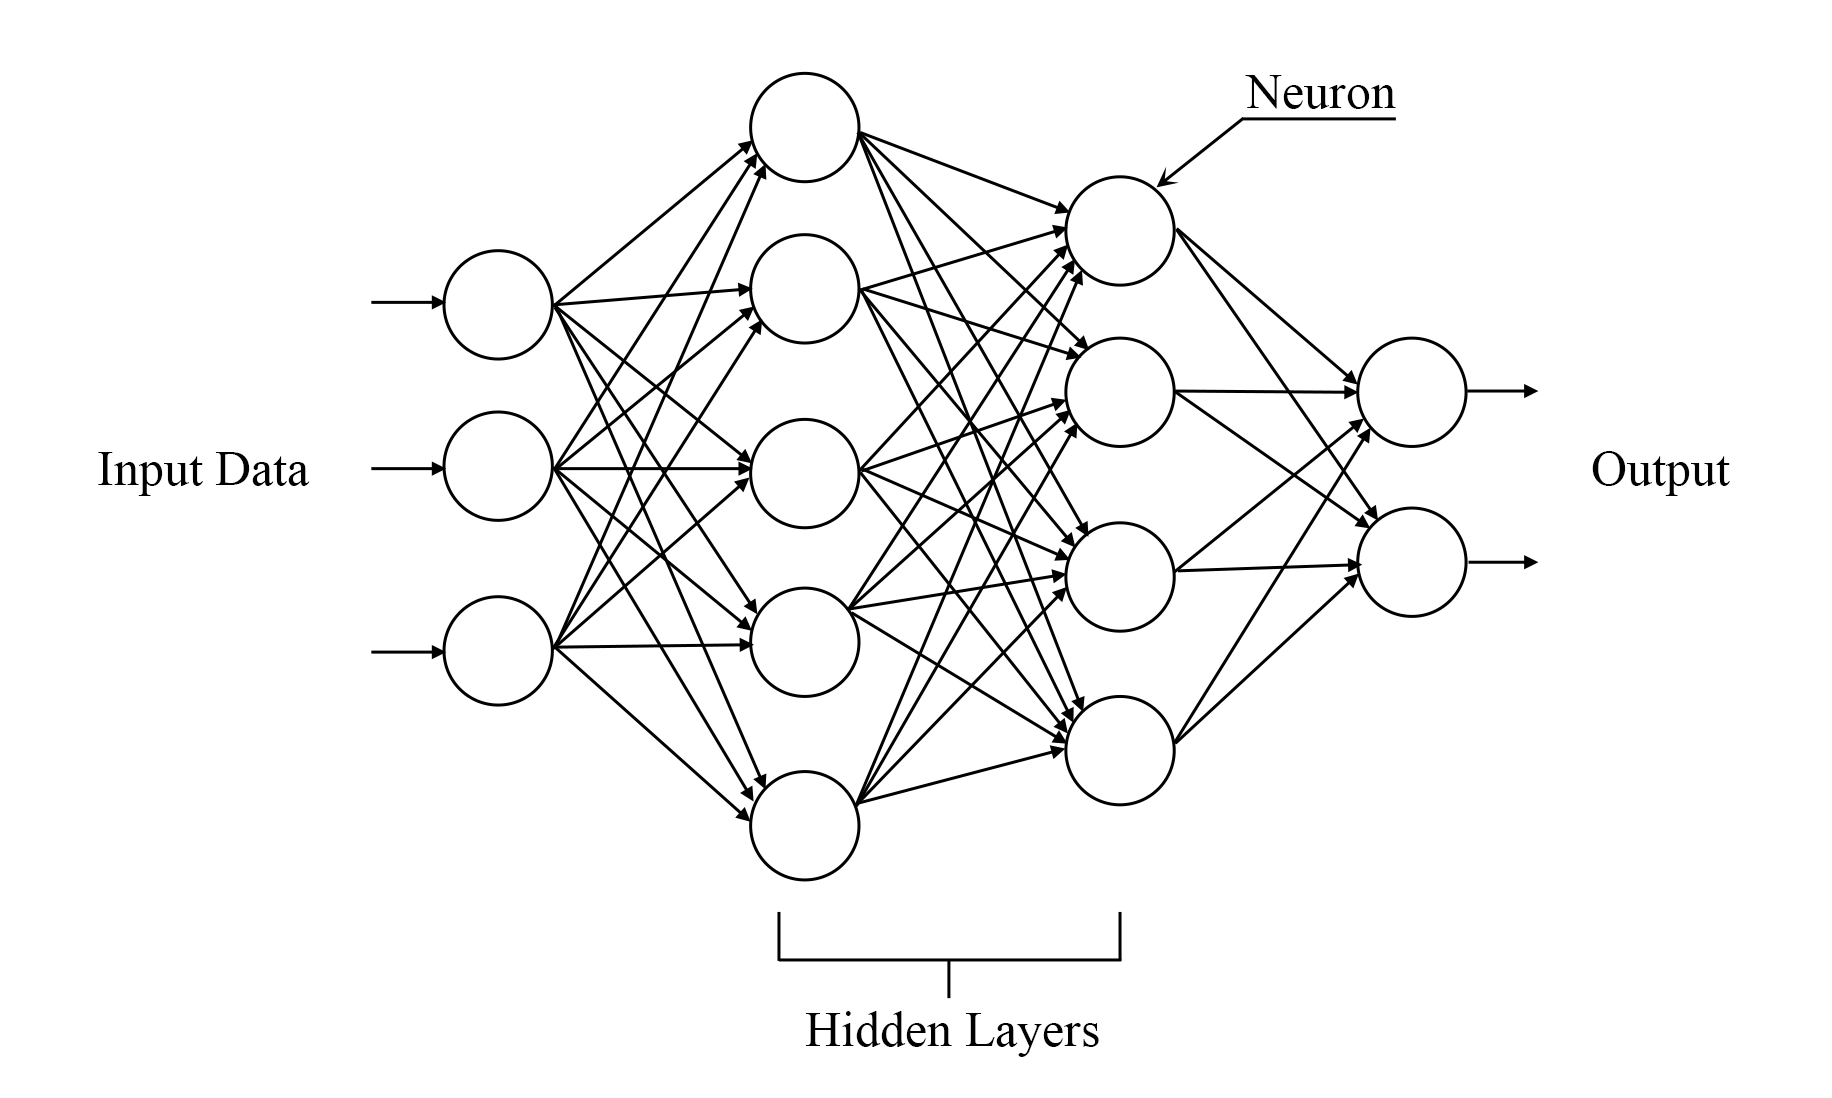
\includegraphics[width=0.8\textwidth]{images/NN.png}
\end{figure}



\subsubsection*{3. Model Training}
\noindent During this stage, we undergo the processes involved in training a model using the concept of \textbf{supervised learning algorithms.}

\noindent This stage can be divided into three sections:
\begin{enumerate}
  \item Data Shuffling
  \item Data Repetition
  \item Training the Model
\end{enumerate}


\begin{itemize}
  \item \underline{Data Shuffling}

    \begin{itemize}
      \item In data shuffling, the prepared dataset is shuffled internally along with their corresponding labels to prevent the model from memorizing the values and give a false sign of higher accuracy, resulting in improper model learning.
      \item This is achieved by using batch-wise shuffling as defined by the 'batch\_size' and 'SHUFFLE\_BUFFER\_SIZE' parameters in the shuffle function used on the dataset.
      \item This process is repeated multiple times during the training process as the shuffle function is called at the end of each epoch of the training cycle.
    \end{itemize}

  \item \underline{Data Repetition}
    \begin{itemize}
      \item In data repetition, the dataset is made to repeat itself multiple times as defined by its function parameters.
      \item This is very useful at times when you wish to test the model with a small dataset size to verify the training process.
    \end{itemize}

  \item \underline{Train Model}
    \begin{itemize}
      \item In the training phase, the prepared dataset is applied to the created model in the previous sections for training.
      \item The training process is carried out by the applied optimizer and loss functions to regulate the learning rate of the model, simultaneously metrics parameters are extracted for model analysis by the user.
      \item Once the model is trained, using the metric parameters (accuracy) and loss function values retrieved during the training process are used to plot the accuracy v/s epoch and loss v/s epoch plots for graphical analysis of the trained model
      \item Model training is achieved by the use of the command 'model.fit()' along with its attributes such as 'epoch=15', target input, and target\_label.
    \end{itemize}

\end{itemize}



\subsubsection*{4. Model Evaluation - Getting Testing Dataset}
\begin{itemize}
  \item In model evaluation phrase, a small portion of unused training dataset is used to evaluate the response of the model to unknown data input.
  \item This phrase also provides to give a test pilot run of the model for its actual implementation output response
  \item Model evaluation is achieved by the use of the command 'model.evaluate()' along with its attributes such as test\_input and target\_label.
\end{itemize}

\subsubsection*{5. Model Saving}
\begin{itemize}
  \item   In model saving, the created and trained model is saved in their individual folder name which is given as its parameter.
  \item   This is achieved by the use of the function 'model.save()'. The weights of the trained model, if needed, can also be stored separately in the form of pickle files. The stored weights can later be used to create or re-train another neural network.
\end{itemize}

\subsection{Classifier Implementation}
\begin{figure}[H]
  \centering
  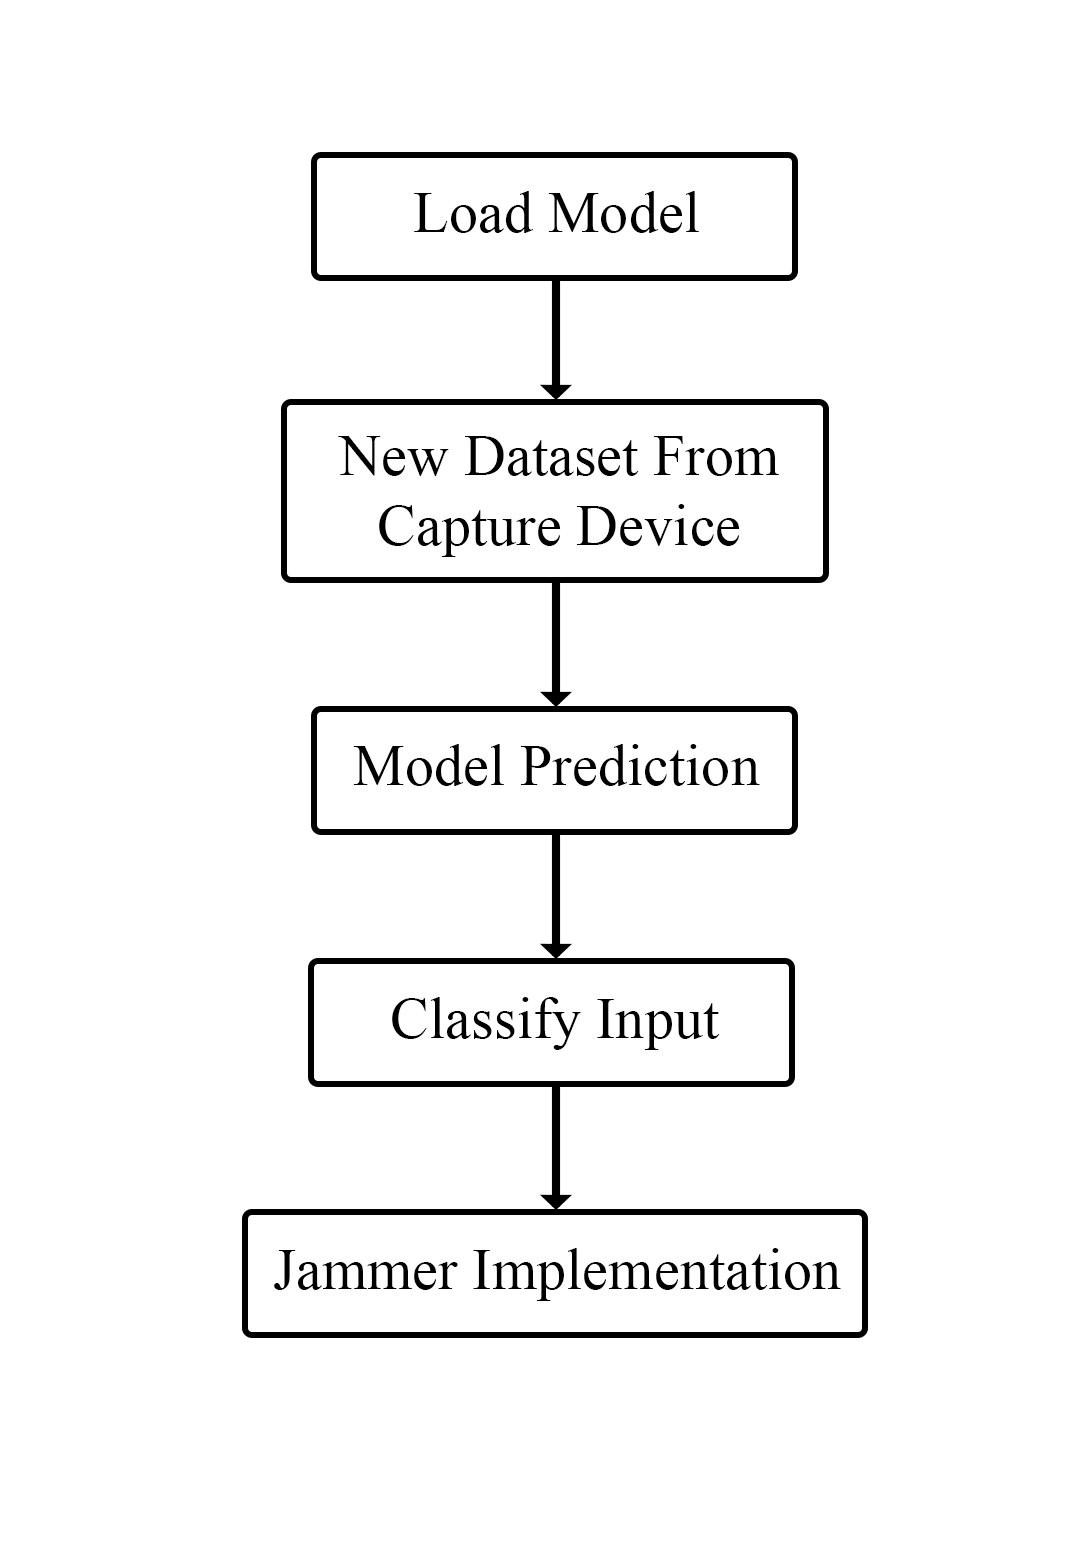
\includegraphics[width=0.5\textwidth]{ Model implementation.png }
  \caption{Classifier Implementation}

\end{figure}
  \subsubsection*{Model Loading}
    \begin{itemize}
      \item Once the entire model is trained, tested and saved in the file system, it needs to be loaded again by a detection code to use the model. This allows for a faster process as the model need not be trained multiple times as the detection process is carried out.
      \item Once the model is loaded, it can perform all the operations a model is able to do after training i.e weight calculation, model evaluation, model prediction and model re-training if needed.
      \item This is achieved by using the function 'models.load\_model()' under the Keras or tensorflow.keras library depending on the version of tensorflow used. Given that the parameter passed to the function is the folder name of the intended model that is to be loaded by the code.
    \end{itemize}

  \subsubsection*{Testing new Dataset from PlutoSDR}
    \begin{itemize}
      \item DataFrame captured by the SDR, that are stored in '.csv' format, are loaded in the code by the use of function 'read\_csv()' under the Pandas Library in Python.
      \item Once the intended DataFrame is loaded, the necessary input signal values are extracted from the DataFrame and stored in the predict\_features variable for the prediction process.
      \item Following the data extraction process, the prediction process begins with appropriate data type and input size arrangements in order to ensure proper prediction.
    \end{itemize}

  \subsubsection*{Model Prediction }
    \begin{itemize}
      \item During the prediction process, the model with its trained weights and algorithm of prediction, tries to predict what output category the given input comes under.
      \item Depending on its classification criterion, it predicts the output category and gives the appropriate probability matrix as its output containing the probability of the input falling under a certain category trained by the model to classify into.
    \end{itemize}


  \subsubsection*{Input Classification}
    \begin{itemize}
      \item In the classification phrase, the output probability matrix of the model is taken and aggregation is performed on the matrix giving a single value as its output.
      \item This singular integer value corresponds to the category predicted by the model. Thus providing the make of the target drone to the jammer system implementation.
    \end{itemize}

  \subsubsection*{Jamming}
    \begin{itemize}
      \item Once the signal is classified into its corresponding make, the code jumps to the corresponding jammer code for that drone maker.
      \item Since the input signal is of a fixed length and in a predefined frequency range, depending on the presence of signal in the captured dataset, the required frequency band and channel can be identified
      \item By using the above two inferences, a suitable and appropriate jamming signal can be transmitted by the jamming transmitter in order to jam/immobilise the target drone communication channels
    \end{itemize}

